\section{System Overview of the LBDT Framework}\label{sec:method_overview}
\noindent The Lightweight Blockchain-Based Data Trading (LBDT) framework is designed to provide secure, low-latency, and incentivized vehicular data exchange in dynamic Internet of Vehicles (IoV) environments. LBDT integrates five core architectural modules: (1) a Dual Parallel Chain Ledger Structure, (2) an Aged Gompertz Reputation Model enhanced by a Machine Learning Honesty Classifier, (3) a Reputation-Aware Double Auction Engine with Bid Loss Penalties, (4) an EC-VRF Leader Election and Gosig BFT Consensus Engine, and (5) a Dynamic Geographic Zone Sharding mechanism.

Figure~\ref{fig:lbdt_flowdiagram} illustrates the complete end-to-end data trading and consensus workflow in LBDT.


\begin{figure}[h!]
\centering
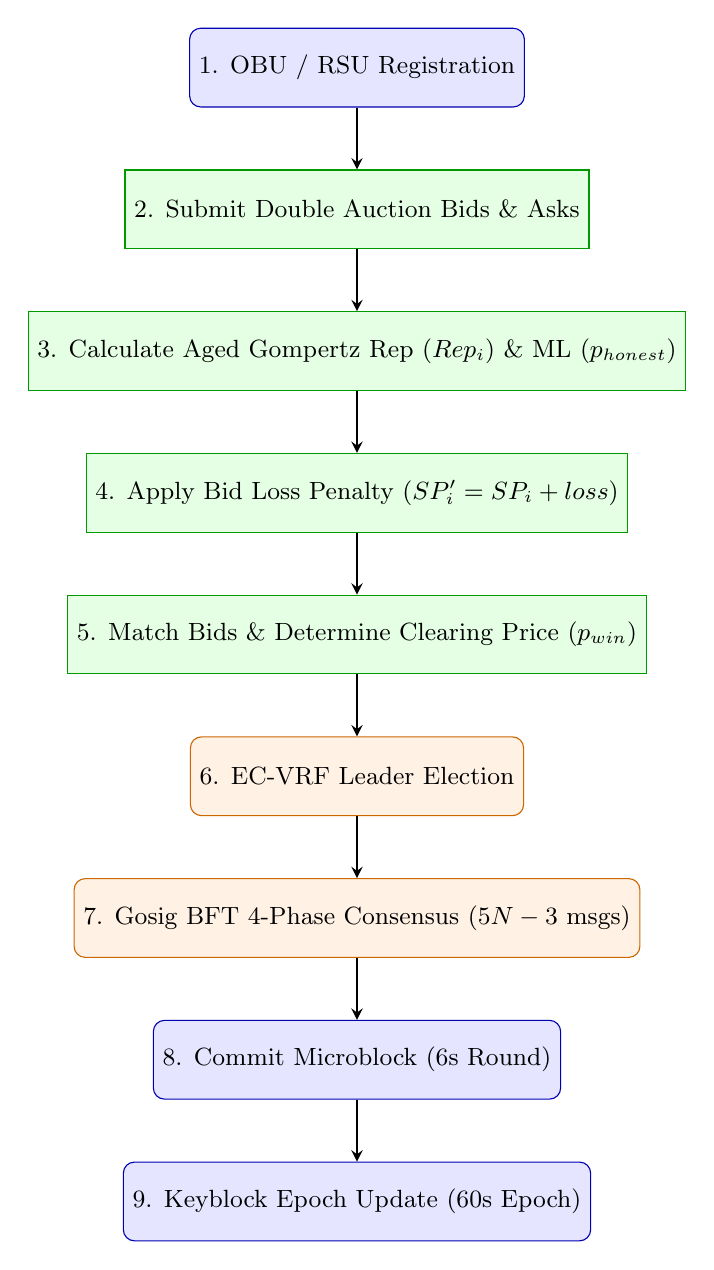
\begin{tikzpicture}[node distance=1.8cm and 2.5cm, auto]
% Styles
\tikzstyle{block} = [rectangle, draw=blue!70!black, fill=blue!10, rounded corners, minimum width=3.2cm, minimum height=1cm, text centered, font=\small]
\tikzstyle{process} = [rectangle, draw=green!60!black, fill=green!10, minimum width=3.2cm, minimum height=1cm, text centered, font=\small]
\tikzstyle{consensus} = [rectangle, draw=orange!80!black, fill=orange!10, rounded corners, minimum width=3.2cm, minimum height=1cm, text centered, font=\small]
\tikzstyle{arrow} = [thick,->,>=stealth]

% Nodes
\node (reg) [block] {1. OBU / RSU Registration};
\node (auc) [process, below of=reg] {2. Submit Double Auction Bids \& Asks};
\node (rep) [process, below of=auc] {3. Calculate Aged Gompertz Rep ($Rep_i$) \& ML ($p_{honest}$)};
\node (loss) [process, below of=rep] {4. Apply Bid Loss Penalty ($SP'_i = SP_i + loss$)};
\node (match) [process, below of=loss] {5. Match Bids \& Determine Clearing Price ($p_{win}$)};

\node (vrf) [consensus, below of=match] {6. EC-VRF Leader Election};
\node (bft) [consensus, below of=vrf] {7. Gosig BFT 4-Phase Consensus ($5N-3$ msgs)};
\node (micro) [block, below of=bft] {8. Commit Microblock (6s Round)};
\node (key) [block, below of=micro] {9. Keyblock Epoch Update (60s Epoch)};

% Arrows
\draw [arrow] (reg) -- (auc);
\draw [arrow] (auc) -- (rep);
\draw [arrow] (rep) -- (loss);
\draw [arrow] (loss) -- (match);
\draw [arrow] (match) -- (vrf);
\draw [arrow] (vrf) -- (bft);
\draw [arrow] (bft) -- (micro);
\draw [arrow] (micro) -- (key);

\end{tikzpicture}
\caption{End-to-End Workflow of the LBDT Data Trading and Consensus Protocol.}
\label{fig:lbdt_flowdiagram}
\end{figure}

\section{Dual Parallel Chain Ledger Architecture}\label{sec:method_dual_chain}
\noindent Traditional blockchain architectures struggle under high vehicular mobility due to the serial block creation bottleneck. LBDT resolves this by decoupling transactions into two distinct block structures:

\begin{enumerate}
    \item \textbf{Microblocks (Trading Chain):} High-frequency, localized blocks generated every short round interval ($\tau_{micro} = 6\text{ seconds}$). Microblocks pack data trading transactions, signed bids, matched clearing prices, and cryptographic data payload hashes. Microblocks require lightweight Gosig BFT validation to minimize latency.
    \item \textbf{Keyblocks (Macro Chain):} Epoch-level management blocks generated every macro epoch ($\tau_{key} = 60\text{ seconds}$). Keyblocks record global node reputation states, active RSU cluster topologies, zone sharding updates, and cryptographic proof anchor roots. Keyblocks use Proof-of-Work (PoW difficulty = 2) for macro-state finality.
\end{enumerate}

\section{Aged Gompertz Reputation \& Machine Learning Classifier}\label{sec:method_reputation}
\noindent To quantify node trustworthiness dynamically, LBDT introduces an Aged Gompertz Reputation Model. For any vehicular node $i$, the aged interaction score $r_n$ accumulates historical transaction feedback while decaying past interactions exponentially:

\begin{equation}
r_n = \left( \sum_{k=1}^{N_{trades}} \gamma^{n - 1 - k} \cdot \delta_k \right) \cdot \ln(N_{peers})
\end{equation}

\noindent where $\gamma = 0.95$ represents the aging decay factor, $\delta_k \in \{+1, -1\}$ denotes positive or negative transaction feedback, $n$ is the current transaction sequence index, and $N_{peers}$ is the total number of distinct trading partners.

The base reputation score $Rep_i$ is governed by a modified Gompertz sigmoidal growth function:

\begin{equation}
Rep_i = a_{adapt} \cdot \exp\left( - b_{adapt} \cdot \exp\left( - c \cdot r_n \right) \right)
\end{equation}

\noindent where $c = 0.1$ is the growth rate constant. To counteract adaptive malicious strategies (e.g., oscillating between honest and dishonest trades), LBDT incorporates a Logistic Regression ML classifier. The classifier evaluates a 4-dimensional telemetry feature vector $\mathbf{x}_i$:

\begin{equation}
\mathbf{x}_i = \left[ \text{honest\_trades}_i, \; \text{cheated\_trades}_i, \; \text{norm\_drop\_rate}_i, \; \text{bft\_responses}_i \right]^T
\end{equation}

The predicted honesty probability $p_{honest} = \sigma(\mathbf{w}^T \mathbf{x}_i + b)$ adaptively adjusts the Gompertz structural parameters:

\begin{align}
a_{adapt} &= a \cdot p_{honest} \qquad (a = 1.0) \\
b_{adapt} &= b + 3.0 \cdot (1 - p_{honest}) \qquad (b = 1.0)
\end{align}

If a node behaves maliciously, $p_{honest} \to 0$, causing $a_{adapt} \to 0$ and $b_{adapt} \to 4.0$, which instantly depresses $Rep_i$ to near zero.

\section{Reputation-Aware Double Auction Mechanism}\label{sec:method_auction}
\noindent Data trading within each zone is settled via a reputation-aware double auction. Data buyers submit bids $BP_j = (v_j, p_j^{\text{bid}})$, and data sellers submit asks $SP_i = (v_i, p_i^{\text{ask}}, \Delta t_i)$. To prevent low-reputation or high-latency sellers from exploiting the market, seller ask prices are adjusted by a bid loss penalty function:

\begin{equation}
loss_i = \alpha_1 \cdot (\Delta t_i)^{\beta_1} + \alpha_2 \cdot (1 - Rep_i)^{\beta_2}
\end{equation}

\noindent where $\alpha_1 = 0.5, \beta_1 = 1.2, \alpha_2 = 1.0, \beta_2 = 2.0$, and $\Delta t_i$ represents the sensor data generation delay. The adjusted seller price $SP'_i$ is formulated as:

\begin{equation}
SP'_i = SP_i + loss_i
\end{equation}

Buyers are sorted in descending order of $BP_j$, and sellers are sorted in ascending order of $SP'_i$. The matching engine identifies the maximum index $m$ satisfying $BP_m \ge SP'_m$. The unified transaction clearing price $p_{win}$ is calculated as:

\begin{equation}
p_{win} = \min\left( BP_m, \; SP'_{m+1} \right)
\end{equation}

\section{EC-VRF Leader Election and Gosig BFT Consensus}\label{sec:method_consensus}
\noindent To achieve lightweight consensus without $O(N^2)$ message overhead, LBDT executes consensus in two steps:

\begin{enumerate}
    \item \textbf{EC-VRF Leader Election:} Committee nodes generate a verifiable random hash $H_{vrf} = \text{VRF\_Hash}(SK_i, seed)$ over the SECP256k1 elliptic curve using $seed = \text{SHA256}(\text{last\_keyblock} \parallel \text{step} \parallel \text{zone\_id})$. The node with the minimum $H_{vrf}$ value is elected consensus leader.
    \item \textbf{Gosig BFT Protocol:} The leader broadcasts the candidate microblock. Consensus proceeds across 4 phases: \textit{Proposal}, \textit{Prepare}, \textit{Tentative Commit}, and \textit{Commit}. By leveraging aggregate multisignatures, total message complexity is strictly bounded to:
    \begin{equation}
    M_{bft} = 5N - 3
    \end{equation}
    where $N$ is the number of active committee RSUs.
\end{enumerate}

\section{Dynamic Geographic Zone Sharding}\label{sec:method_sharding}
\noindent To handle fluctuating vehicle densities across urban corridors, LBDT implements dynamic geographic sharding. Each zone $z_p$ continuously calculates a utility load score $U_z$:

\begin{equation}
U_z = 0.3 \left( \frac{V_z}{V_{max}} \right) + 0.3 \left( \frac{T_{wait}}{T_{limit}} \right) + 0.4 \cdot R_{adv}
\end{equation}

\noindent where $V_z$ is vehicle count, $T_{wait}$ is average transaction queueing delay, and $R_{adv}$ represents adversarial node ratio. When $U_z > 0.85$, the zone automatically splits into sub-zones. Conversely, when $U_z < 0.20$, adjacent sparse zones merge.

\section{C++ Veins to Python Simulation Architecture}\label{sec:method_integration}
\noindent The system implementation couples the C++ OMNeT++/Veins discrete-event network simulator (\texttt{LBDTApp.cc}) with a Python backend server (\texttt{socket\_server.py}) over a low-latency TCP socket protocol (port 8000). The C++ module captures SUMO mobility events, generates V2X wireless packets, and delegates auction matching, machine learning classification, and blockchain ledger commits to Python in real time.